\documentclass{article}
\usepackage[margin=2cm,nomarginpar]{geometry}
\usepackage[T1]{fontenc}

\usepackage{graphicx}
\usepackage{url}
\usepackage{hyperref}
\graphicspath{ {./images/} }

\usepackage{listings}
\lstdefinestyle{mystyle}{
	basicstyle=\ttfamily\footnotesize,
	breakatwhitespace=false,
	breaklines=false,
	captionpos=b,
	keepspaces=true,
	showspaces=false,
	showstringspaces=false,
	showtabs=false,
	tabsize=2
}
\lstset{style=mystyle}

\title{Java+MIDI: Synthesizer und Drum-Machines per Code steuern}

\begin{document}
	
	\begin{center}
		\includegraphics[width=.1\textwidth]{images/hawlogo.png}
		\\
		\LARGE Java+MIDI: Synthesizer und Drum-Machines per Code steuern\\
	\end{center}
	
	\section{Instrumente}
	In diesem Workshop verwenden wir zwei Arten von elektronischen Instrumenten:
	\begin{itemize}
		\item \textbf{Synthesizer}: Erzeugen Noten, für Melodien oder Basslinien.
		\item \textbf{Drum-Machines}: Erzeugen Percussion Sounds, z.B. den Beat in einem Song.
	\end{itemize}
	
	\section{MIDI}
	MIDI (Musical Instruments Digital Interface) ist ein Standard, mit dem elektronische Musikinstrumente Informationen austauschen.
	Diese Kommunikation geschieht in Form von \textbf{Messages}.
	Eines solche Message besteht aus einer definierten Anzahl an Bits (0 oder 1), die dann interpretiert werden.
	
	\begin{tabular}{l|l}
		\textbf{Bit Nummer} & \textbf{Bedeutung} \\
		0-3 & Art der Nachricht \\
		4-7 & MIDI Channel \\
		8-15 & Note \\
		16-23 & Velocity \\
	\end{tabular}
	
	\subsection{MIDI Channel}
	Midi Channel werden genutzt, um Nachrichten an ein bestimmtes Gerät zu schicken:\\
	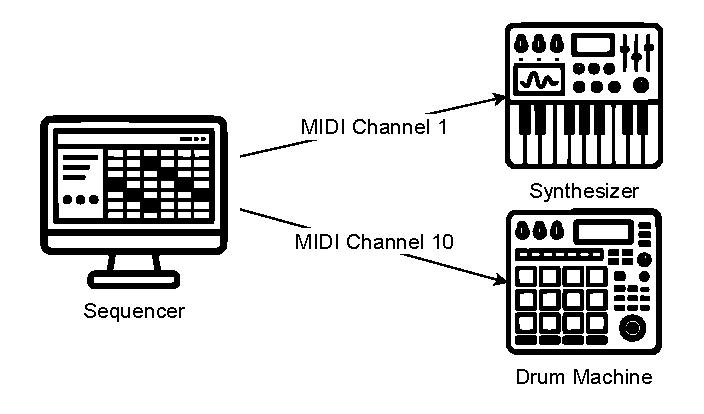
\includegraphics[width=.5\textwidth]{images/setup.pdf}
	\begin{itemize}
		\item \textbf{Sequencer:} Sendet MIDI Nachrichten
		\item \textbf{Drum Machine:} Empfängt MIDI Nachrichten mit MIDI Channel 10 und spielt entsprechende Drum Sounds.
		\item \textbf{Synthesizer:} Empfängt MIDI Nachrichten mit MIDI Channel 1 und spielt entsprechende Synthesizer Sounds.
	\end{itemize}
	
	\subsection{NOTE ON}
	Eine NOTE ON Message weißt ein MIDI Gerät an, eine bestimmte Note abzuspielen.
	Zum Beispiel:
	
	\begin{tabular}{l|l}
		\textbf{Bits} & \textbf{Bedeutung} \\
		1001 & NOTE ON \\
		0000 & MIDI Channel 1\\
		11111111 & Note 127 \\
		11111111 & Velocity 127 (so laut wie möglich) \\
	\end{tabular}
	
	\subsection{NOTE OFF}
	Eine NOTE OFF Message weißt ein MIDI Gerät an, eine bestimmte Note zu stoppen.
	Zum Beispiel:
	
	\begin{tabular}{l|l}
		\textbf{Bits} & \textbf{Bedeutung} \\
		1000 & NOTE OFF \\
		0000 & MIDI Channel 1\\
		11111111 & Note 127 \\
		11111111 & Velocity 127 (unwichtig) \\
	\end{tabular}
	
	\subsection{NOTE Tabelle}
	Die Bedeutung der Note (0-127) kann folgender Tabelle entnommen werden:\\
	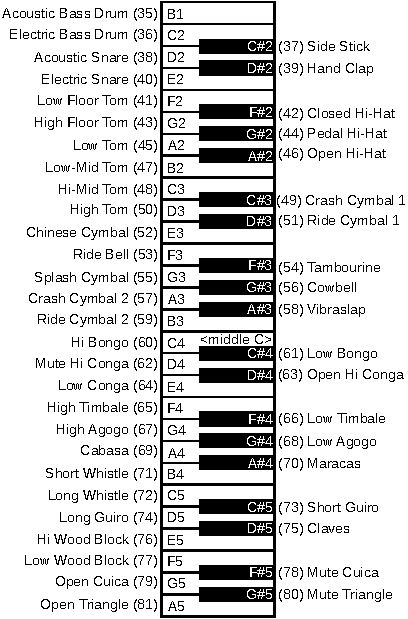
\includegraphics[width=.5\textwidth]{images/drumMap.pdf}
	\\
	Beispiele:
	\begin{itemize}
		\item Wird die Note 57 an einen Synthesizer gesendet, spielt dieser die Note "A3"
		\item Wird die Note 57 an eine Drum Machine gesendet, spielt diese den Sound "Crash Cymbal 2" 
	\end{itemize}
	
	\newpage
	\section{MIDI + Java}
	Die Programmiersprache Java stellt einfache Funktionalitäten bereit, MIDI Nachrichten an angeschlossene Geräte zu senden.
	Zusätzlich verfügt Java über einen "eingebauten" Synthesizer und eine eingebaute Drum Machine.
	Auf Ihrem Rechner finden Sie folgendes Beispielprogramm:
	\lstinputlisting{../src/main/java/Main.java}
	Dieser Beispielcode macht folgendes:
	\begin{itemize}
		\item Erzeugung eines Objektes der Klasse "JavaAndMidi".
		Dise gibt Ihnen die Möglichkeit, über den Synthesizer Channel oder Drum Machine Channel Noten und Percussion abzuspielen.
		\item Speichern des Midi Channels für die Drum Machine in die variable \verb|drumChannel|.
		\item Speichern des Midi Channels für den Synthesizer in die variable \verb|synthesizerChannel|.
		\item Abspielen eines Drum Sounds.
		\item Abspielen eines Synthesizer Sounds.
	\end{itemize}
	
	\subsection{NOTE ON}
	Eine Note wird folgendermaßen abgespielt:
\begin{lstlisting}
myChannel.noteOn(35, 127);	
\end{lstlisting}
	
	\subsection{NOTE OFF}
	Eine Note wird folgendermaßen gestoppt:
\begin{lstlisting}drumChannel.allNotesOff();
myChannel.noteOff(35, 127);	
\end{lstlisting}
	Sie können aber auch alle Noten auf dem betreffendem Channel stoppen:
\begin{lstlisting}
myChannel.allNotesOff();	
\end{lstlisting}

	\subsection{Warten}
	Damit eine Note auch Zeit hat um zu klingen, muss zwischen NOTE ON und NOTE OFF eine Pause stattfinden:
\begin{lstlisting}
myChannel.noteOn(35, 127);
javaAndMidi.sleep(500);
myChannel.allNotesOff();	
\end{lstlisting}

	\subsection{Loops}
	In Java können mit den Schlüsselwörtern \verb|for| können Schleifen erstellt werden.
	Alles was innerhalb den geschweiften Klammern der Schleife steht wird wiederholt:
\begin{lstlisting}
for (int i = 0; i < 10; i++) { // tue stuff 10 mal
	// stuff
}
\end{lstlisting}

	\section{Aufgaben}
	Jetzt, da Sie die Basics kennen, legen Sie mit folgenden Aufgaben los:
	\begin{enumerate}
		\item Führen sie das Beispiel Programm aus, es sollte eine Bass Drum und eine Syntesizer Note abgespielt werden.
		\item Verändern Sie den Sound, der von der Drum Machine abgespielt wird.
		\item Nutzen Sie eine Schleife, um die Sounds 100 mal abzuspielen.
		\item Verändern Sie die Wartezeit, um das Abspielen schneller oder langsamer zu machen.
		\item Erstellen Sie einen typischen Schlagzeug Rhythmus. Typische Rhythmen finden Sie unter \ref{rhythmen}.
		\item \textbf{Have Fun}: Erstellen Sie ihren eigenen Song :).
	\end{enumerate}
	\textbf{TIPP:} Duplizieren Sie für jede Aufgabe die Datei Main, damit sie den Beispielcode und ihre vorherigen Aufgaben immer als Vorlage bereit haben.
	
	\section{Rhythmen}\label{rhythmen}
	\subsection{Standard Rythmus}
	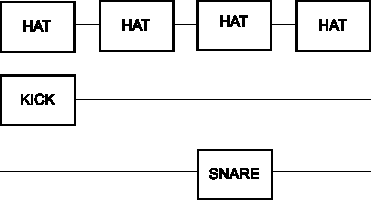
\includegraphics[height=.18\textheight]{images/standard.pdf}	
	\subsection{Drum And Bass}
	\includegraphics[height=.18\textheight]{images/drumAndBass.pdf}
	\subsection{House}
	\includegraphics[height=.18\textheight]{images/house.pdf}
\end{document}




